% !TeX spellcheck = en_US
% !TeX encoding = UTF-8
% !TeX root = ../thesis.tex

\chapter{How to Use This Template}

In this chapter, the features of this template will be explained.


\section{Language}\label{s:language}

The language of this template is \texttt{english}. This is the default language of all works at ALR. Only switch to German after talking to your supervisor(s)!

To switch use the  \texttt{\textbackslash{}selectlanguage} macro in \texttt{thesis.tex}.
If you write your thesis in German instead, set the language to \texttt{ngerman}.
After switching the language, delete all auxiliary files.


\section{Data Configuration}

In \Cref{tab:macros}, the macros to configure the meta data in this document are listed.
The macros should be set in the preamble of \texttt{thesis.tex}.

\begin{table}[ht!]
\caption{Macros available in this template to configure the document.}
\vspace*{0.5cm}
\centering
\begin{tabular}{ll}
\toprule
Macro & Description \\
\midrule 
\texttt{\textbackslash mythesis} & Use one of \texttt{\textbackslash mastersthesis}, \texttt{\textbackslash bachelorsthesis}, \\
& \texttt{\textbackslash termpaper} \emph{(Seminararbeit)}, \texttt{\textbackslash protocol} \\
\texttt{\textbackslash myname} & \emph{Your full name} \\
\texttt{\textbackslash mytitle} & \emph{Title of your thesis} \\
\texttt{\textbackslash myshorttitle} & \emph{Subtitle of your thesis (optional)} \\
\texttt{\textbackslash timestart} & \emph{Begin of your thesis} \\
\texttt{\textbackslash timeend} & \emph{End of your thesis} \\
\texttt{\textbackslash referee} & \emph{Referee} \\
\texttt{\textbackslash refereetwo} & \emph{Second referee (only if needed)} \\
\texttt{\textbackslash refereethree} & \emph{Third referee (only if needed)} \\
\texttt{\textbackslash advisor} & \emph{Advisor} \\
\texttt{\textbackslash advisortwo} & \emph{Second advisor (only if needed)} \\
\texttt{\textbackslash advisorthree} & \emph{Thrid advisor (only if needed)} \\
\bottomrule
\end{tabular}
\label{tab:macros}
\end{table}


\section{References}

To reference another section, chapter, etc., this template makes use of \href{https://ctan.org/pkg/cleveref?lang=en}{cleveref}.
For example, to refer to the language section in this chapter, use \texttt{\textbackslash{}Cref\{s:language\}}, which results in: \Cref{s:language}.


\section{Citations}

For citations, you should use Bibtex together with \href{https://www.ctan.org/pkg/natbib}{natbib}.
If you want, you can also use BibLaTeX instead.

Test second citation: \citet{kober2013reinforcement}

For most purposes, \texttt{\textbackslash{}citet} can be used to produce references like this: \citet{deisenroth2013survey}.
If you want to list all authors, the asterisk version \texttt{\textbackslash{}citet*} can be used to produce such references: \citet*{deisenroth2013survey}.
If you want the reference to be in parentheses, \texttt{\textbackslash{}citep} can be used: \citep{deisenroth2013survey}.

It is \emph{most important} that you abide by scientific standards to cite correctly.
Read and comply with the \href{https://www.kit.edu/downloads/gute_wiss_praxis_en.pdf}{rules for safeguarding good scientific practice at Karlsruhe Institute of Technology} (German original:  \href{https://www.sle.kit.edu/downloads/AmtlicheBekanntmachungen/2018_AB_032.pdf}{\textit{Satzung zur Sicherung guter wissenschaftlicher Praxis am Karlsruher Institut für Technologie}}).
In case of uncertainty, consult your advisor.


\section{Tables}

For an example table, please refer to \Cref{tab:macros}.
It is generally advised to use the \href{https://ctan.org/pkg/booktabs?lang=en}{booktabs} package for good looking tables.
The most important paradigms on making tables are that you should never use vertical rules, and you should never use double rules.
Refer to the manual of this package for the reasoning or rationale of these paradigms, and also for examples on how to properly design tables.


\section{Figures}

In \Cref{fig:example}, you can see an example figure of some robots.

\begin{figure}[ht!]
    \centering
    \subfigure[Robot]{\label{fig:example}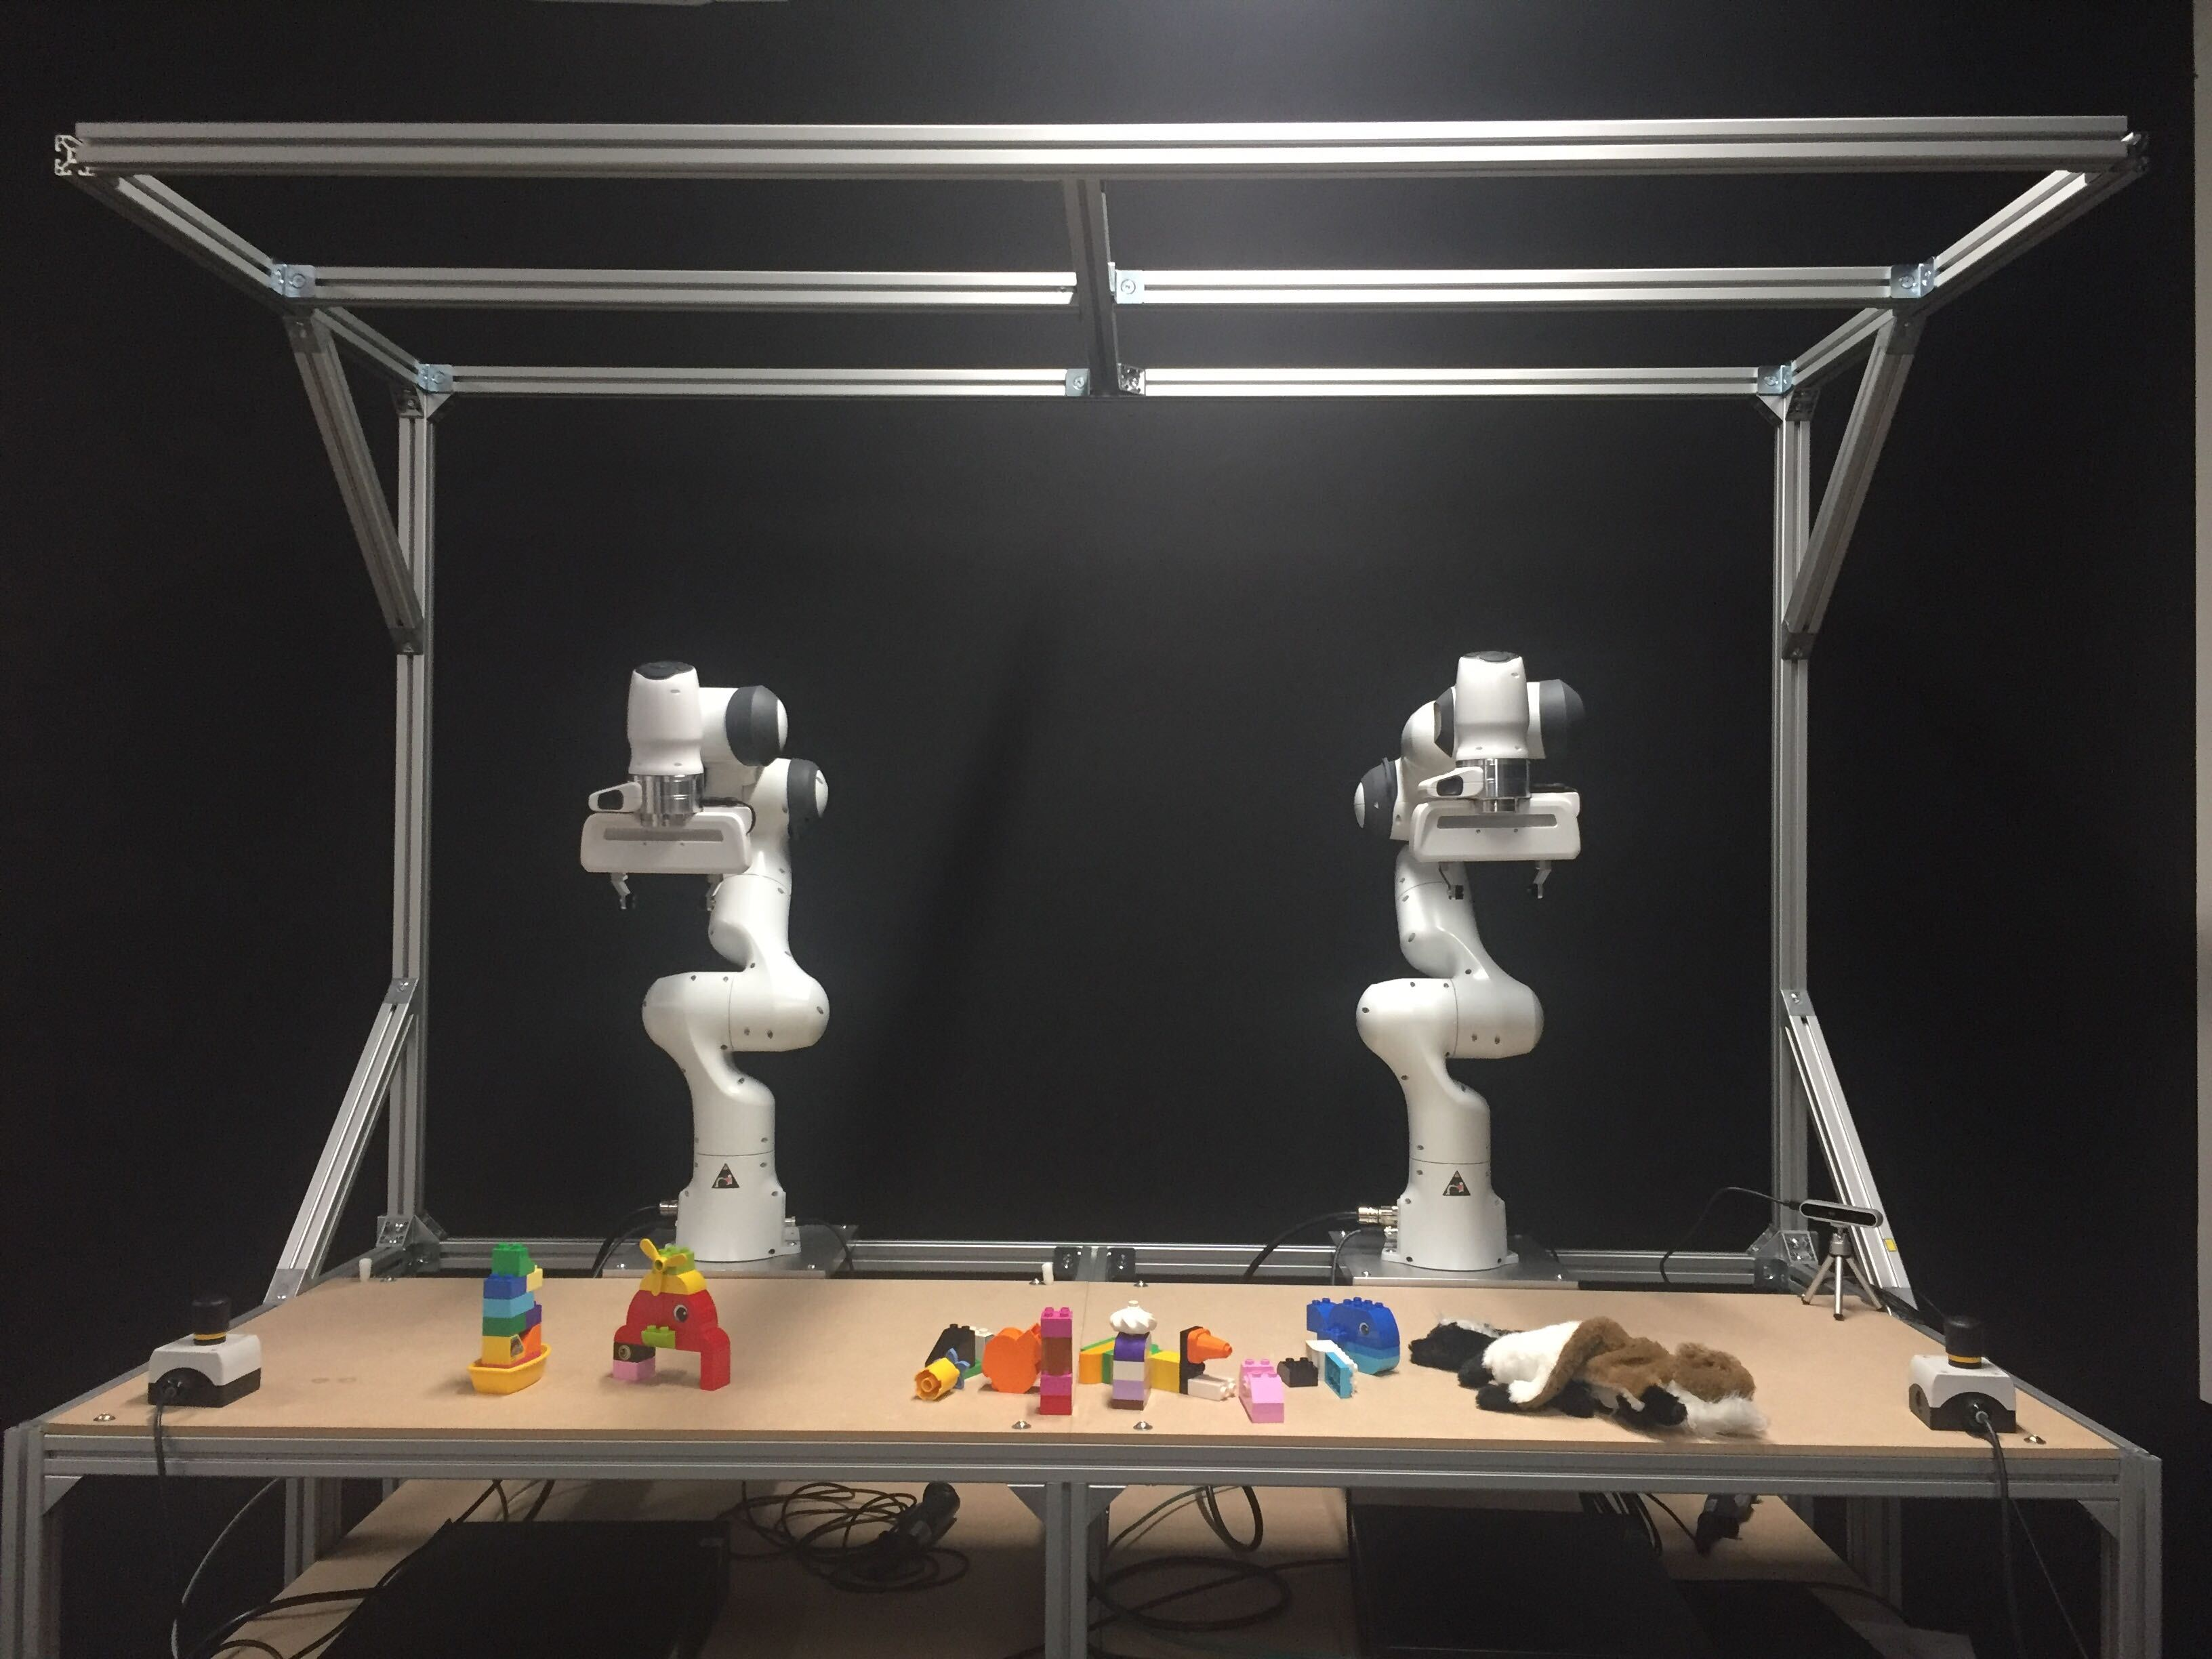
\includegraphics[width=0.4\textwidth]{figures/robot}}    
    \hspace{1cm}                       
    \caption{Robots with squeaky dog toys}
    \label{fig:example}
\end{figure}

Please use vectorgraphics (pdf, eps, svg, see also tikzplotlib) for all plots in your thesis.  


\Cref{fig:svgexample} shows an SVG file rendered in the document as vector graphic using the \href{https://ctan.org/pkg/svg?lang=en}{svg} package.
This requires to have Inkscape installed, and \texttt{pdflatex} needs to be called together with the \texttt{-{}-shell-escape} option.

\begin{figure}[ht!]
    \centering
    \includesvg[width=0.5\textwidth]{figures/vector_graphic}
    \caption{Example SVG rendered in \LaTeX{} as vector graphic.}
    \label{fig:svgexample}
\end{figure}

